\subsection{Modeling the R-Transform}
\label{sxn:r_transforms}

\charles{NOTE: There is some subtly here to deal woith because of the branch cuts expected in $R(z)$
  We can derive \ALPHAHAT from the R-Transform, but its a bit lengthy.
  I will also work out the R transform for the truncated power law for $\alpha=2$ and maybe $3,4$ and explain}

\iffalse
PREVIOUS:
In this section, we explain how to select the \RTransform $R(z)$ and evaluate the~\GEN~$\GN$ under different modeling assumptions.
To apply \SETOL, the model satisfy the \TRACELOG condition--which occurs during the case of  \IdealLearning.
For most cases of NN models, the ESD are HT; and this, in practice, one usually would select $R(x)$ that reflects this. 
We analyze several cases, noting their applicability to real-world scenarios.
Most importantly,  we derive expressions that resemble the~\WW~\ALPHAHAT metric, at least formally valid
for the case $\alpha\approx 2$.
\fi

In this section, we explain how to select the \RTransform $R(z)$ and evaluate $\GN$ and thus $\QT$ under different modeling assumptions.
Recall that, to apply \SETOL, the model satisfy the \TRACELOG condition.
We analyze several cases, noting their applicability to real-world scenarios.

(((For most cases of NN models, the ESD are HT; and this, in practice, one usually would select $R(x)$ that reflects this.)))

(((Most importantly,  we derive expressions that resemble the~\WW~\ALPHAHAT metric, at least formally valid
for the case $\alpha\approx 2$.)))


%%\subsubsection{Elementary Random Matrix Theory}
%%\label{sxn:r_transforms:elementary_rmt}
\paragraph{Elementary Random Matrix Theory Notation.}

We begin with some useful notions from \RandomMatrixTheory.
%
Using the ESD, $\rho(\lambda)$, defined as
\begin{equation}
\label{eqn:rgo}
\rho(\lambda):=\frac{1}{N}\sum_{i}\delta(\lambda-\lambda_{i})  ,
\end{equation}
%
we can express the \emph{\GreensFunction}%
\footnote{Note our naming and sign convention; some authors equate the \GreensFunction $G(z)$ with
the \Cauchy-Stieltjes transform, whereas we define $C(z)=-G(z)$. 
\michaelB{QUESTION @charles: Say why; is this to be consistent with Zee, or Burda.}
}
(or \emph{\Cauchy}-Stieltjes transform) by%
\begin{equation}
\label{eqn:Gz}
G(z):=\int \mathrm{d}\lambda \frac{\rho(\lambda)}{z-\lambda} .
\end{equation}
%
From $G(z)$, we can recover the ESD, $\rho(\lambda)$, using the inversion relation
%\begin{equation}
%\label{eqn:GzInverse}
%\rho(\lambda)=\lim_{\epsilon\rightarrow 0+}\frac{1}{\pi}\mathrm{IM}(C(\lambda+i\epsilon))  ,
%\end{equation}
\begin{equation}
\label{eqn:GzInverse}
\rho(\lambda)=\lim_{\epsilon\rightarrow 0+}\frac{1}{\pi}\mathrm{Im}(G(\lambda+i\epsilon))  ,
\end{equation}
% MM NOT: I CHANGED C TO G TO FIZ THE TYPO.
where 
%%$\mathrm{IM}$
$\mathrm{Im}(\cdot)$
takes the imaginary part of the input, and where the $\lim_{\epsilon\rightarrow 0+}$ means to take the limit approaching from the upper half of the complex plane.
\michaelB{NOTE: I changed ``IM'' to be ``Im'' to be more standard; this is the only place it appears, aside from in misc/all\_equations.tex, so we need to change it there unless that is a derived file.}
%
The \RTransform, $R(z)$, can be defined using the Blue function,%
\footnote{The Blue function was first introduced by Zee~\cite{Zee1996} to model, among other things, spectral broadening in quantum systems.
%Briefly, given a deterministic Hamiltonian matrix $\mathbf{H}_{0}$, with eigenvalues $\lambda^{0}_{i}$, one can model the spectral broadening of $\lambda^{0}_{i}$ by adding a random matrix $\mathbf{H}_{1}$ to $\mathbf{H}_{0}$: $\mathbf{H}=\mathbf{H}_{0}+\mathbf{H}_{1}$.  
%The resulting eigenvalues of $\mathbf{H}$ now contain some level of randomness, $\sigma$, i.e., $\lambda=\lambda^{0}+\sigma$.  
%To model the ESD of $\mathbf{H}$, one then specifies the invididual \RTransforms for $\mathbf{H}_{0}$ and $\mathbf{H}_{1}$; the full ESD of $\mathbf{H}$ can then be reconstructed by adding the two \RTransforms together $R(z)=R_{0}(z)+R_{1}(z)$.
Zee also notes that $R(z)$ is the same as the self-energy $\Sigma(z)$ from quantum many body theory~\cite{Zee1996}.
This provides an interesting interpretation to our main results. }
$B(z)$, as 
\begin{equation}
\label{eqn:Rz}
R(z):=B(z)-\frac{1}{z}  ,
\end{equation}
where $B(z)$~\cite{Zee1996} is the functional inverse of the Greens Function, $G(z)$,
satisfying 
\begin{equation}
\label{eqn:GzRelation}
B[G(z)]=z  .
\end{equation}
Thus, by specifying the complete \RTransform, $R(z)$, we specify the complete ESD, $\rho(\lambda)$.
Here, we are actually only interested in the tail of the ESD, $\rho_{tail}(\lambda)$.
That is, if $R(z)=R_{tail}(z)+R_{bulk}(z)$, then we only need $R_{tail}(z)\approx R(z)$.
\charles{Describe $R(z)$ is a power series, and how we take $\int dz R(z)$ and why we restirct the integral, contours, etc}
\michaelB{Maybe yes (to the commented out comment about power series); see some of the additional cols/rows I put in  the table; let's sync.}


%%\subsubsection{Known \RTransforms and Analytic (Formal) Models}
%%\label{sxn:r_transforms:known_r_transforms}

There are only a few models for which analytic results for $R(z)$ are known.
See Table~\ref{tab:known_r_transforms} for a summary.
Below, we review several of them, explaining the ESD to which they correspond,
and what the resulting $G(\lambda)$ would be if applied
as a model $R(x)$ in the \SETOL approach.
\michaelB{MM TO DO: Reword.}


\begin{table}[h!]
  \centering
  \renewcommand{\arraystretch}{1.25} % Increase line spacing in table
\begin{tabular}{|c|c|c|c|c|}
  \hline
  Model & XXX & \HTSR Universality class & \RTransform $R(z)$  
  \\  \hline
  \hline
  Discrete Spikes & XXX & Spikes & $\tfrac{1}{\MECS}\sum_{i=1}^{\MECS}\lambda_{i}$  
  \\  \hline
  \hline
%  Wishart Models & XXX & &  
%  \\  \hline
  \InverseWishart & XXX & HT/VHT &  $\dfrac{\kappa-\sqrt{\kappa(\kappa-2z)}}{z}$  
  \\  \hline 
  Multiplicative-Wishart & XXX & HT/VHT& $\dfrac{\epsilon\phi z^2}{2 - \epsilon\phi^2 z^2}$ 
  \\  \hline
  \hline
%  Levy \Wigner & XXX &   &  
%  \\  \hline
  Levy \Wigner: General  $(\alpha_{l}\ne 1)$ & XXX & VHT/HT  & $a+bz^{\alpha_{l}-1}$ 
  \\  \hline
  Levy \Wigner: \Cauchy $\alpha_{l}=2, \beta=0$ & XXX & $\alpha=2$ & $a - i\gamma$ 
  \\  \hline
\end{tabular}
\caption{Known \RTransforms for different matrix models.
  The \emph{Multiplicative-Wishart} model has two real, non-zero parameters, $\epsilon$ and $\phi$; for more details, see \cite{Pennington2017}.
  For the \emph{\InverseWishart}, as given by Bun~\cite{BunThesis}, $\kappa=\frac{1}{2}(Q-1)$ where, $q=\frac{1}{Q}=\frac{M}{N}\le 1$.
  The \emph{\LevyWigner} model describes \Wigner-like Square Random Matrices
  (as opposed to Wishart-like or Correlation Matrices), where the elements are drawn from a Levy-Stable distribution.
  The Levy-Stable $R(z)$ is parameterized by a (real) shift parameter $a$,
  a complex phase factor $b$ (that depends on 3 real parameters  $\alpha_{l}, \beta$, and $\gamma$),
  and, importantly,  a PL-like tail exponent $\alpha_{l}\in (0,2)$;
  For more details, the text, see~\cite{BJNx01_TR,BJNx06_TR,BJ09_TR}.
  \red{For our modeling purposes here, we make the association $\alpha_{l}\sim\alpha/2-2$. maybe not?}
  (Also, for simplicity, we assume the variance $\sigma=1$ for all models above, where appropriate.)
  \michaelB{QUESTION @charles: What is the ref with the general form for $\sigma$.}
  \nred{Note: removed \emph{Multiplicative-Wishart} Might want to comment on it.  MM TO DO: PUT IT BACK. } \charlesB{SEE RTable.tex.  MERGE}
}  
\label{tab:known_r_transforms}
\end{table}

1;95;0c% Rtable.tex
\begin{table}[h!]
  \centering
  \renewcommand{\arraystretch}{1.25} % Increase line spacing in table
\begin{tabular}{|c|c|c|}
  \hline
  Model & \textbf{HTSR Universality Class} & \textbf{$R(z)$}\\  \hline
  \hline
  Discrete & Bulk$+$Spikes, MHT, HT & $\tfrac{1}{\MECS}\sum_{i=1}^{\MECS}\lambda_{i}$   \\ \hline
  \hline
  Wishart Models & &\\ \hline
  Multiplicative-Wishart & HT/VHT& $\dfrac{\epsilon\phi z^2}{2 - \epsilon\phi^2 z^2}$ \\  \hline
  Inverse Marchenko-Pastur & HT/VHT &  $\dfrac{\kappa-\sqrt{\kappa(\kappa-2z)}}{z}$   \\  \hline
  \hline
  L\'evy Wigner (LW) &   & \\  \hline
  Free Cauchy (FC) ($\alpha_{l}=1$) & HT $\alpha=2$ & $a+i\gamma$ \\ \hline
  General L\'evy  ($\alpha_{l}\ne 1$) & VHT $\alpha<2$   & $a+bz^{\alpha-2}$ \\  \hline
\end{tabular}
  \caption{Known \RTransforms for random matrix ensembles relevant to modeling heavy-tailed spectral densities (eigenvalues or singular values squared).
    The \emph{Multiplicative-Wishart} model has two real, non-zero parameters, $\epsilon$ and $\phi$; for more details,
    see \cite{PW16_NIPS}.
  For the \emph{\InverseMP}, as given by Bun~\cite{BunThesis}, $\kappa=\frac{1}{2}(Q-1)$ where, $q=\frac{1}{Q}=\frac{M}{N}\le 1$.
  The \emph{L\'evy-Wigner} (LW) model describes Wigner-like square random matrices
  (as opposed to Wishart-like or Correlation Matrices), where the elements are drawn from a L\'evy-Stable distribution.
  The resulting LW ESD is Heavy-Tailed Power Law, and characterized by the L\'evy exponent $\alpha_{l}$.
  The LW $R(z)$ is parameterized by a (real) shift parameter $a$,
  a complex phase factor $b$ (that depends on 3 real parameters   $\alpha_{l}, \beta$, and $\gamma$),
  and, of course, $\alpha_{l}$.
  The Free Cauchy (FC) model is a special case of the IW model, corresponding to the L\'evy $\alpha_{l}=1$, and the \HTSR $\alpha=2$. 
  We will extend the LW models to the rectangular case for our modeling purposes here by making
  the association   $\alpha = \alpha_{l}+1$ for $\alpha\le 2$.
  %$\alpha=\tfrac{1}{2}(\alpha_{l}+1)+1$ for $\alpha\le 2$.
   (Also, wwe take thew variance $\sigma=1$ for all models.)
   Generally speaking, the L\'evy $R(z)$ are more complicated; 
   for more details, see~\cite{BJNx01_TR,BJNx06_TR,BJ09_TR}.
}
\label{tab:known_r_transforms}
\end{table}



\charles{Discuss the Table briefly, and then each model in its own subsubsection.
We can create plots to show how these models can treat heavy tails, and explain the parameter fitting
}



%\subsubsection{Discrete Model: Spikes}
\paragraph{Discrete Independent Spikes.}

Here, we consider modeling the tail of the ESD, $\rho_{tail}(\lambda)$, as a collection of discrete (independent) spikes $\lambda_{i}^{(spike)}$, where $\lambda_{i}^{(spike)}\ge \LambdaECSmin$.
While this model is not very realistic, we include it as a baseline.
%%(((
%%For this model, the \RTransform for the \ECS is sum of Dirac delta functions.
%%\michaelB{QUESTION @charles: Clarify.  Is that right?  Or are the eigenvalues spikes, and the R-transform is constant over some (complex) domain (where the constant is the sum of the eigenvalues in the ECS)?}
%%)))
This lets us compute the \LayerQuality $\Q$ in closed form in terms of properties of the Teacher weight matrix, $\TMAT=\WMAT$.

To do so, let the tail of the ESD have 
%%$\MECS = M^{tail}$ 
$\MECS$ 
eigenvalues, $ \left\{ \lambda_i \right\}_{i=1}^{\MECS}$, all such that $\lambda_{i}\ge \LambdaECSmin$, that define the \ECS, i.e.,  
\begin{equation}
\label{eqn:spikes_model_0}
\rho_{tail}(\lambda)=\sum_{i=1}^{\MECS}\delta(\lambda-\lambda_{i}) .
\end{equation}
\michaeladdressed{Let's sync, since I don't know what that phrase means in this context, and I want to make sure we didn't introduce a confusion above.}
\charles{@michael: seriously?!  We have discussed this multiple times.  We dicussed it at dinner in New Orleans.}
The \GreensFunction $G(z)$ is then
\begin{equation}
\label{eqn:spikes_model_1}
G(z) = \int d\lambda \dfrac{ \rho_{tail}(\lambda) }{z - \lambda} 
     = \sum_{i \in \ECS} \int d\lambda \dfrac{\delta(\lambda-\lambda_{i})}{z - \lambda} 
     = \sum_{i \in \ECS} \dfrac{1}{z-\lambda_{i}}  ,
\end{equation}
where we have used the notation $i \in \ECS$ to refer to the $\MECS$ eigenvalues that specify the \ECS.
Observe that for each individual term in the sum, $\frac{1}{z-\lambda_{i}}$, the Blue function is $B(z) = \lambda_{i}+\frac{1}{z}$.
Thus, using the additive property of the \RTransform, we can express the total $R(z)$ as the sum of the \RTransforms for the individual terms $i$, giving
\begin{equation}
\label{eqn:spikes_model_2}
R(z) =\sum_{i\in\ECS}\left(\lambda_{i}+ \dfrac{1}{z}\right) - \dfrac{1}{z}=
\sum_{i\in\ECS}\lambda_{i}  .
\end{equation}
\michaelB{why do we not get $\MECS-1$ copies of $\frac{1}{z}$?}
\charlesB{This is the definition}
From this, we can express $\GN$ as
\begin{align}
\label{eqn:spikes_model_3} 
\GN 
%&
= \int_{\LambdaECSmin}^{\lambda}\sum_{i\in\ECS}\lambda_{i} d\lambda 
%\\ \nonumber
%&
= \sum_{i\in\ECS}\lambda_{i} \int_{\LambdaECSmin}^{\lambda} 1 d\lambda 
%\\ \nonumber
%&
= \left(\sum_{i\in\ECS}\lambda_{i}\right)\left(\lambda-\LambdaECSmin\right)
\approx \left(\sum_{i\in\ECS}\lambda_{i}\right)\left(\lambda\right) ,
\end{align}
where the last approximation holds under the assumption that $\LambdaECSmin \ll \lambda$ (which typically holds).
%Seeing that $\LambdaECSmin$ is usually quite small, we make the approximation
%\begin{align}
%\GN  \approx \left(\sum_{i}\lambda_{i}\right)\left(\lambda\right)  ,
%\end{align}
This expression holds in particular for every eigenvalue $\lambda_i$ in the \ECS.
To evaluate the \QualitySquared approximately, $\QT$, we must sum this quantity over every eigenvalue in the \ECS, as
\begin{align}
  \label{eqn:spikes_model_4}
  \QT = \sum_{i\in\ECS}\GNI 
 \approx \sum_{i\in\ECS}\left(\sum_{i^{\prime}\in\ECS}\lambda_{i^{\prime}}\right)\left(\lambda\right)
 = \left(\sum_{i\in\ECS}\lambda_{i}\right)^{2}  .
\end{align}
Thus, $\Q:=\sqrt{\QT}=\sum_{i\in\ECS}\lambda_{i}$.
Being the sum of the top $\MECS$ eigenvalues of a Hermitian matrix, this quantity is a matrix norm; and thus $\Q$ can be approximated as a ``tail norm.''
\michaelB{MM TO DO: Check symmetric vs spsd issue.}


%The Multiplicative-Wishart (MW) model  has two real, adjustable parameters $\epsilon,\phi$.
%It treates $\mathbf{X}$ as resulting from product of random matrices, and is good for modeling an ESD with a very heavy tail.
%It has been used previously to model the heavy tail of the Hessian matrix in NNs\cite{Pennington2017}
%This model would work better for fitting HT ESDs that decay slower than a TPL.  We will not consider
%this model further here and leave this for future work.

%We will work out  the full details, going from $\rho(\lambda)\rightarrow G(z)\rightarrow R(z)\rightarrow \QT$

\charlesB{ADD THIS SECTION, moce some stuff around:
\paragraph{Free Cauchy Model.}
Here, we can obtain the expression for $\QualitySquared\approx\lambda_{max}\sim\frac{1}{\alpha}$
This is formally correct but the Levy model ($\beta=0$) is not a great model for real world ESDs
}
\michaelB{Yes, agreed, I think Inverse Wishart should be last.}

%%\subsubsection{Inverse-Wishart Model of \IdealLearning}
\paragraph{Inverse-Wishart Model.}

Here, we consider the \InverseWishart (IW) model.
The IW model treats the ESD of $\mathbf{X}^{-1}$, when the ESD of $\mathbf{X}$ itself is MP.

As a parametiric model, it can be quite effective at treating VHT and HT (or \FatTailed) ESDs when the far tail decays very rapidly, like a TPL, and/or for $\alpha\le 4$.
To do this, one simply considers the parameters $\kappa$ as an adjustable paremeter.
\michaeladdressed{Give a functional form, with $\kappa$ appearing.}
\charles{@michael: do it yourself or don't suggest it}
%
It is an excellent model for the ESD when $\alpha=2.0$ (and $Q=2$).
Using this model, we can derive an expression for the \HTSR \ALPHAHAT \LayerQuality metric,
$\ALPHAHATEQN :=\ALPHAHATLONG)$ as a leading order term in the final expression for $\log_{10}\QT$.

This model 

\michaelB{Redo below, after go through derivation in the appendix.}

\begin{figure}[h]
    \centering
    \subfigure[IW Distribution, $\kappa=0.25$]{ 
      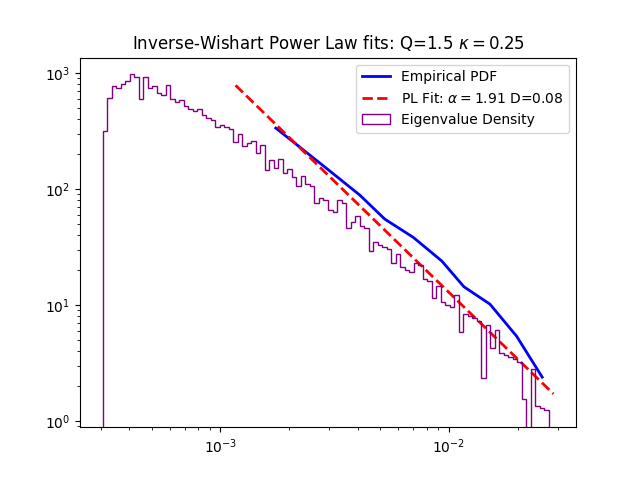
\includegraphics[width=5cm]{./img/IWplotQ1.5.png}
      \label{fig:IWplotQ15}                                                                                                      
    }                               
      \subfigure[IW Distribution, $\kappa=1.25$]{ 
      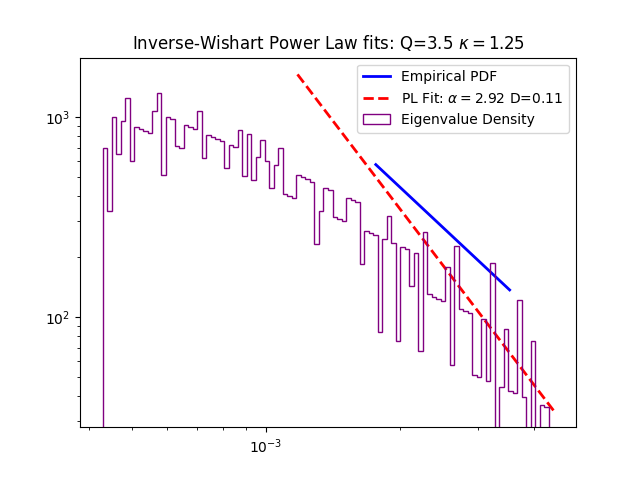
\includegraphics[width=5cm]{./img/IWplotQ3.5.png}
      \label{fig:IWplotQ35}                                                                                                      
      }
      \caption{Example Inverse-Wishart (IW) distributions for $\kappa=0.25$ and $\kappa=1.25$,  along with Power Law (PL) fits of the generated distribution. Plots on Log-Log scale.}
  \label{fig:IWplots}                                                                                                      
\end{figure}   

In Figure~\ref{fig:IWplots}, we fit some \Typical layer ESDs to an IW distribution.
When $\kappa=0.25$, the fitted $\alpha=1.91$, and the fit is a reasonably accurate model of the underlying Power Law
distribution and the ~\WW PL fit.
For  $\kappa=1.25$, the fitted $\alpha=2.92$ is larger, but the fit is not as good as a
model. Generally speaking, $\alpha$ scales with $\kappa$, but the  free cumulants scale inversely with $\kappa$.
So smaller $\alpha$ will give larger free cumulants and therefore a larger $\QT$.
Importantly, as seen in Figure~\ref{fig:IWplotQ15}, for $\alpha=\simeq 2.0$, the IW model (with $\kappa=0.25$)
is an effective simple model to illustrate the \SETOL case of \IdealLearning.
\michaeladdressed{Maybe this par and fig elsewhere; or at end of subsubsxn.}
\charles{@michael: low priority; can revisit}

\begin{figure}[t]
    \centering
    \subfigure[IW $R(z)$, real $z$.]{
        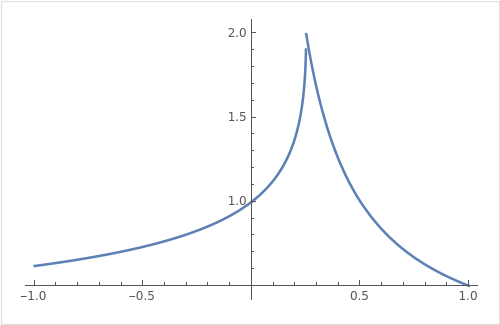
\includegraphics[width=4cm]{./img/R.png}
        \label{fig:IW_R}
    }
    \subfigure[Branch cut at $z=\kappa/2$]{
        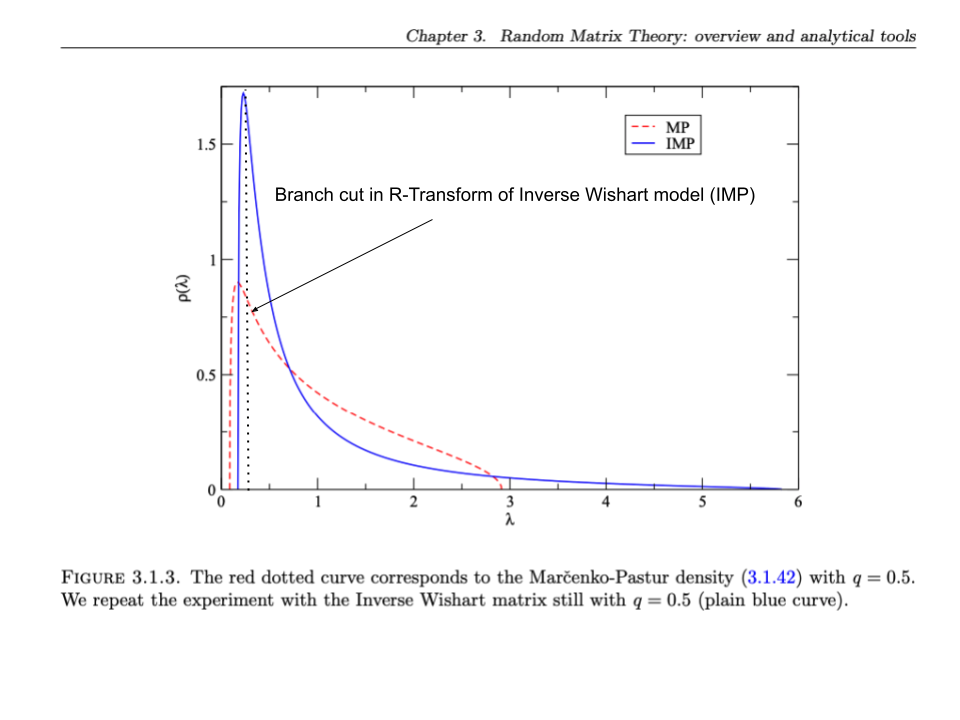
\includegraphics[width=4cm]{./img/branch-cut.png}
        \label{fig:IW_branch_cut}
    }
    \caption{(a) The function $R(z)$ of the Inverse Wishart model, with a singularity at $z = \kappa/2$. (b) The branch cut in the empirical spectral density, corresponding to the tail for $\kappa = 0.5$.}
    \label{fig:R_branch_cut_combined}
\end{figure}

Lets consider $R(z)$ for the \InverseWishart model, denoted $R(z)[IW]$.
To integrate this function, we require that it be analytic.
At first glance, it may seem that that $R(z)[IW]$ is not analytic because it
has a pole at $z=0$ and because the square-root term $\sqrt{\kappa(\kappa-2z)}$  creates branch
cut at and $z=\kappa/2$ (and $z=\infty$).
Figure~\ref{fig:R_branch_cut_combined} presents this in two ways:
Figure~\ref{fig:IW_R} shows the R-transform $R(z)[IZ]$ for real $z$, highlighting its singular behavior and the location of the branch cut at $z = \kappa/2$; and
Figure~\ref{fig:IW_branch_cut} shows the corresponding branch cut in the ESD of the Inverse Wishart model (for $\kappa = 0.5$).
We select the branch cut starting at $z=\kappa/2$ and ending at $z=\infty$,
which allows us to at least formally defined the integral along the physically meaningful part of the ESD:
\begin{equation}
\label{eqn:IW_model_1} 
\GN[IW] := \int_{\LambdaECSmin}^{\lambda} R(z)[IW] dz  ,
\end{equation}
noting that we expect $\LambdaECSmin\ge\kappa/2$.
\michael{Why do we have this par, if we are using quality squared. I need to understand.}
\charles{@michael: whats the issue ?}

It turns out, however, that due to the branch cut in $R(z)[IW]$,
the function $\GN[IW]$ is not analytic in the domain we need. 
To correct for this, we will instead model the \LayerQualitySquared using the modulus of $\GN[IW]$,
\begin{equation}
\label{eqn:IW_model_1} 
|\GN[IW]| := \sqrt{\GN[IW]^{*}\GN[IW]}
\end{equation}
where $\GN[IW]^{*}$ is the complex conjugate of $\GN[IW]$.
This is somewhat involved, so we present the full calculation in Appendix~\ref{sxn:IW}
\michael{MM TO DO: Go through.}
\michael{Are we going to mention the result here since we will use it?}


Figure~\ref{fig:InverseWishartGx} plots $|\GN[IW]|$ on Lin-lin and Log-log plots, on the range $\lambda\in(0.25, 100)$, and fits the it to a PL. 
The fit follows the general trend of the function, but it is not terribly accurate.
Still, from this plot, we can see that the \LayerQualitySquared has the same general trend as $\ALPHAHAT$ and/or a Shatten Norm.

\begin{figure}[t]
  \centering
  \subfigure[$|\GN\lbrack IW\rbrack|$ Lin-lin plot and PL fit]{
    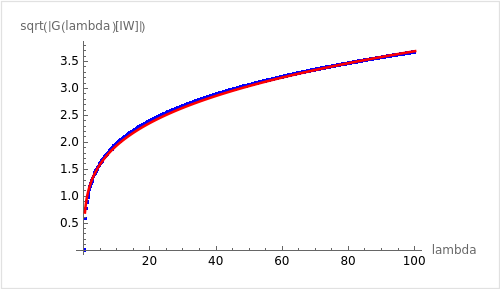
\includegraphics[width=0.45\textwidth]{./img/Gx.png}
        \label{fig:GxPlot}
    }
    \subfigure[$|\GN\lbrack IW\rbrack|$ Log-log plot and PL fit]{
        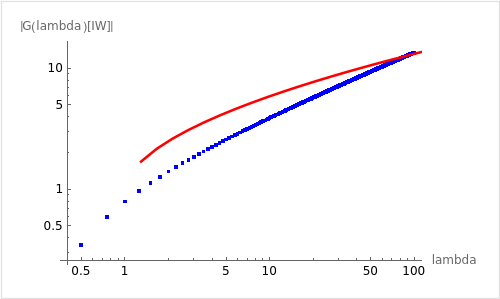
\includegraphics[width=0.45\textwidth]{./img/logGx.png}
        \label{fig:LogLogGxPlot}
    }
    \caption{Behavior of $\GN[IW]$ for the Inverse Wishart (IW) model,
       with a Power Law (PL) fit (red), $|\GN[IW]|\approx 1.138 \lambda^{0.539}$.
      (a)  Lin-lin plot. (b) Log-log plot.
}
    \label{fig:InverseWishartGx}
\end{figure}

%
%\begin{figure}[t]
%    \centering
%    % Subfigure (a): G(x) Plot
%    \subfigure[Inverse Wishart $\GN$]{
%        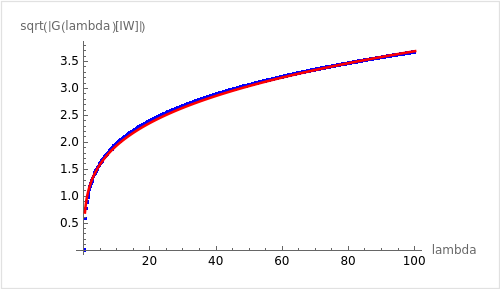
\includegraphics[width=0.45\textwidth]{./img/Gx.png}
%        \label{fig:GxPlot}
%    }
%    % Subfigure (b): Log-log plot and power-law fit
%    \subfigure[Log-log plot and power-law fit]{
%        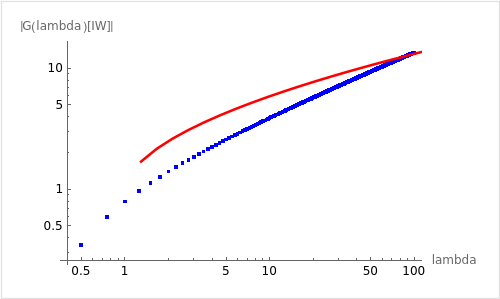
\includegraphics[width=0.45\textwidth]{./img/logGx.png}
%        \label{fig:LogLogGxPlot}
%    }
%    \caption{Behavior of $\GN$ for the Inverse Wishart (IW) model. (a) $\GN$ lin-lin plot. (b) Log-log plot of $\GN$ with a Power Law (PL) fit, $\GN\sim 2.8\lambda^{-3.0}$ }
%    \label{fig:InverseWishartGx}
%\end{figure}
%
%Given an analytic expression for $\GN$ (and $\kappa=0.25$), we can plot the $\GN$ as a function of $\lambda$,
%and then fit this to a Power Law; this is depicted in Figure~\ref{fig:InverseWishartGx}.
%The resulting fit gives $\GN\simeq 2.8\lambda^{3.0}$.
%We can now associate $\ALPHAHAT$ with $\log_{10}\QT$ by keep the leading order term
%$(\lambda_{max}=\LambdaECS_{max}$)
%
%\begin{align}
%  \label{eqn:IW_alphahat}
%  \ALPHAHATEQN:=\ALPHAHATLONG\approx\log_{10}\QT=\log_{10}\sum_{\LambdaECS}\GNI\approx\log_{10}\mathcal{G}(\lambda_{max}\sim (\alpha+1)\log_{10}\lambda_{max}
%\end{align}
%So for $\alpha=2.0$, $\log_{10}\QT\sim (\alpha+1)\log_{10}\lambda_{max}$, which is very close to $\alpha\log_{10}\lambda_{max}$. QED.



%%\subsubsection{Levy-Wigner Models and the \ALPHAHAT Metric}
\paragraph{Levy-Wigner Models.}

Here, we consider Levy-Wigner Models.
We show how to obtain the \WW~\ALPHAHAT metric by modeling the near VHT cases with an approximation to a Levy distribution at $\alpha\approx 2$.  \charlesB{THis is actually for $\alpha \le 2$.  The idea is to correct for correlation traps and another scale anomalies that push $\alpha<2$. In these cases, $\lambda_{max}>1$ so smaller alpha DECREASES the quality.  Also, that in the Nature paper,  we did NOT normalize $\mathbf{W}$ by $\frac{1}{M}$, so we get right trend (but for the wrong reason) Thats science}

We do this because the~\ALPHAHAT metric has been developed to adjust for \SCALE anomalies that arise from issues like \CorrelationTraps,
making \ALPHA smaller than expected.
The  \LevyWigner (LW) model treats  $\mathbf{X}$ as if it were a \Wigner matrix (and not actually a correlation  matrix), and the $\alpha$ is different but related to $\alpha$ above in Table~\ref{tab:known_r_transforms}.
The ESD follows a Levy-Stable distribution, where $a$ is a shift parameter, and $b$ is a complex phase factor depending on 2 real factors, $\beta$ and $\gamma$.
Strictly the ESD for an LW model, $\rho_{LW}(\lambda)$, is defined by its characteristic function (i.e., the Fourier Transform of $\rho_{LW}(\lambda)$), but
we can note that the ESD is VHT, $\rho_{LW}(\lambda)\sim\lambda^{-\alpha-1}$, and that when $\alpha_{l}\approx 1$, the ESD resembles a PL HT ESD with $\alpha\approx 2$.

For case of \IdealLearning,  we choose to \emph{model} the \RTransform of our Fat-Tailed HT ESDs as
\begin{equation}
\label{eqn:LW_model_0} 
R(z)[HT] = bz^{\alpha-1},\;\alpha\simeq 2
\end{equation}
where $b$ is an unspecified constant (possibly negative and/or complex).
\michael{We need to clarify. Are we saying that we do PM instead of LW here.}
Notice that when $\alpha\approx 2$, our model is close to the LW model, $R(z)[HT]\approx R(z)[LW]$
(and gives a \Cauchy distribution if we choose $b=a-i\gamma$).

Integrating $R(z)[HT]$, and (as above) taking the approximation $\LambdaECSmin\sim 0$, we obtain (formally)
\begin{equation}
\label{eqn:LW_model_1} 
\GN[HT] = \tfrac{b}{\alpha} \lambda^{\alpha}  .
\end{equation}
%
If we now choose $b=\alpha=2$, then  $\QT$ takes the form of a Shatten Norm (squared)
\begin{equation}
  \label{eqn:LW_model_2}
  \QT = \tfrac{1}{\MECS}\sum_{i}\lambda^{\alpha}  .
\end{equation}
%
Taking the logarithm of $\GN[HT] $, we obtain
\begin{equation}
\label{eqn:LW_model_3} 
\log \GN[HT] =  \log\tfrac{b}{\alpha} +\tfrac{\alpha}\log\lambda
\end{equation}

As with the \InverseWishart (IW) model, we can derive a formal expression for $\ALPHAHAT$ using the LW model.
To do so, let us approxmate $\QT$ by the largest term in the sum over $\GN$, and then let $\lambda=\lambda_{max}$, giving
\begin{equation} 
\label{eqn:LW_model_4} 
\ALPHAHATEQN = \log_{10} \QT \approx  \alpha\log\lambda_{max}   .
\end{equation}
We present this as a formal example, noting that is slightly different from the result for the IW model, Eqn.~\ref{eqn:IW_alphahat}. 
We do not claim this is a valid empirical model, as we have not attempted to fit a real-world ESD to Levy-stable distribtion.  
\michael{Let's sync on the rationale here, since I'm not sure what is being said.}
We leave this to a future study, noting, however, there has been some work doing such fits~\cite{li2024exploring}.

Ideally, we would like to have an rigorous expression for $R(z)$ not just
in the case of \IdealLearning but also for the entire \FatTailed Universality class.
This is non-trivial to obtain and we will attempt this in a future work.
Fow now, we will take a different approach, and evaluate $R(z)$ explicitly using numerical techniques.

\charlesB{Should summarize somewhere}
\include{sections/GTable}

\subsubsection{Computational Random Matrix Analysis}
\label{sxn:comp_rmt}
\nred{The presence of the branch cut at the start of the ECS complicates this section.
  We may need to remove it entirely as it is probably deeply wrong
  and save it for a future work.  Not super happy about that but time is limitted.
  I will think some more on it
  }
The \RTransform is the generating function for the \emph{\FreeCumulants} of RMT.  Formally, one can define $R(z)$ as a series expansion in $z$,
\begin{equation}
  \label{eqn:Rz_expansion}
  R(z) := \kappa_1 + \kappa_2 z + \kappa_3 z^2 + \ldots 
\end{equation}
where the coefficients $\kappa_{k}$ are the free cumulants, which can be expressed
in terms of the matrix moments $m_{k}$\cite{FreeCumulants}, defined (here) as
\begin{equation}
  \label{eqn:mk_defn}
  m_{k}:=\Trace{\XECS^{k}}=\sum_{i=1}^{\MECS}(\LambdaECS)^{k}
\end{equation}
where $\LambdaECS_{k}$ is the k-th eigenvalue of the effective correlation matrix $\mathbf\XECS$,
which  has been mean-centered and normalized by its standard deviation.

The free cumulants are defined recursively as
\begin{equation}
  \label{eqn:kappa_defn}
  \kappa_k := m_k - \sum_{\text{partitions of } n} \prod_{\text{blocks } B} m_{|B|} 
\end{equation}
\charles{finish explanation}

The first 5 \emph{\Cumulants} are, explicitly,
\begin{align}
  \label{eqn:kappa_defn_2}
  k_1 = m_1 \\ \nonumber
  k_2 = m_2 - m_1^2 \\ \nonumber
  k_3 = m_3 - 3 m_2 m_1 + 2 m_1^3 \\ \nonumber
  k_4 = m_4 - 4 m_3 m_1 - 2 m_2^2 + 10 m_2 m_1^2 - 5 m_1^4 \\ \nonumber 
  k_5 = m_5 - 5 m_4 m_1 + 15 m_3 m_1^2 + 15 m_2^2 m_1 - 35 m_2 m_1^3 - 5 m_3 m_2 + 14 m_1^5
\end{align}

Using these definitions, we can estimate the \LayerQuality matrix $\QT$ for our experimental models
(in Section~\ref{sxn:empirical} by computing  $\GN$ for the effective correlation space
(i.e. the tail of the layer ESD), however it is defined.  That is, we use

\begin{align}
  \label{eqn:G_lambda_series}
\GNI=\kappa_{1}\frac{\LambdaECS}{\MECS}+\frac{\kappa_{2}}{2}\left(\dfrac{\LambdaECS}{\MECS}\right)^{2}+\cdots
\end{align}
Note that we evaluate $\GN$ using eigenvalues normalized with $\tfrac{1}{\MECS}$.
\nred{although this may not be obvious the way we have written things so far}
\charles{We may not need to specify the $\tfrac{1}{\MECS}$ term anymore because I think the code now uses
  the properly normalized $\XECS$, but I need to check carefully}
\charles{Mention experimental section in XXX}



